%!TEX program = xelatex
\documentclass[cn,hazy,blue,14pt,screen]{elegantnote}
\title{Kyrios:平衡机器算法应用运行时工具}

\author{施华}
\institute{Kyrios Algorithm Application Runtime Tool}

\version{beta-0.1}
\date{\zhtoday}

\usepackage{array}

\begin{document}

\maketitle

\centerline{
  
\includegraphics[width=0.2\textwidth]{logo-ae.png}
}



\section{Exia Algorithm Manager介绍}

Kyrios Algorithm Application Runtime Tool主要针对算法开发中算法端生产落地工程化、与后端交互两大方面的一系列问题来设计构建,是一个纯Python语言工具包,采用OOP编程范式,Pythonic代码风格。

Kyrios Algorithm Application Runtime Tool有下面几个特性:

\begin{itemize}
  \item 高度自由可定制
  \item 插件开发度高,可自由组合
  \item 提供功能完善的基础套餐(计算、通信、存储、管理、设计、接口)
\end{itemize}

以下主要是主体框架和基础套餐的设计说明



\subsection{主体框架}

Kyrios Algorithm Application Runtime Tool主要分为三大模块,分为控制、扩展和基础单元。控制模块主要管理算法应用功能的组合与使用;基础模块主要管理算法应用功能的具体实现;扩展模块主要抽象出了可复用的六大基本功能——信息、结构、执行、状态、扩展和接口。三大模块主要涉及的技术有:

\begin{enumerate}[label=\arabic*).]
	\item \textit{命令模式}\\
	主要用于控制模块中自定义组合各自的基础功能单元。
	\item \textit{工厂模式}\\
	主要用于控制模块中生产特定功能单元。
	\item \textit{构建模块}\\
	主要用于控制模块中自定义功能单元的创建过程。
	\item \textit{Ray}\\
	主要用于基础功能模块计算单元,实现分布式计算与各进程间通信。
	\item \textit{Alluxio}\\
	主要用于基础功能模块存储单元,构建数据抽象层,实现数据统一格式,加速IO操作。
	\item \textit{Networkx}\\
	主要用于所有基础单元,为所有功能单元提供一个自定义数据结构的途径,该途径主要基于图论相关。
	\item \textit{transitions}\\
	主要用于所有基础单元,为所有功能单元提供状态监控功能。
	\item \textit{Hydra}\\
	主要用于基础功能模块管理单元,实现脚本动态配置。
	\item \textit{Hydra}\\
	主要用于基础功能模块管理单元,实现代码模板自动生成,高度可配置。	
\end{enumerate}

\centerline{
	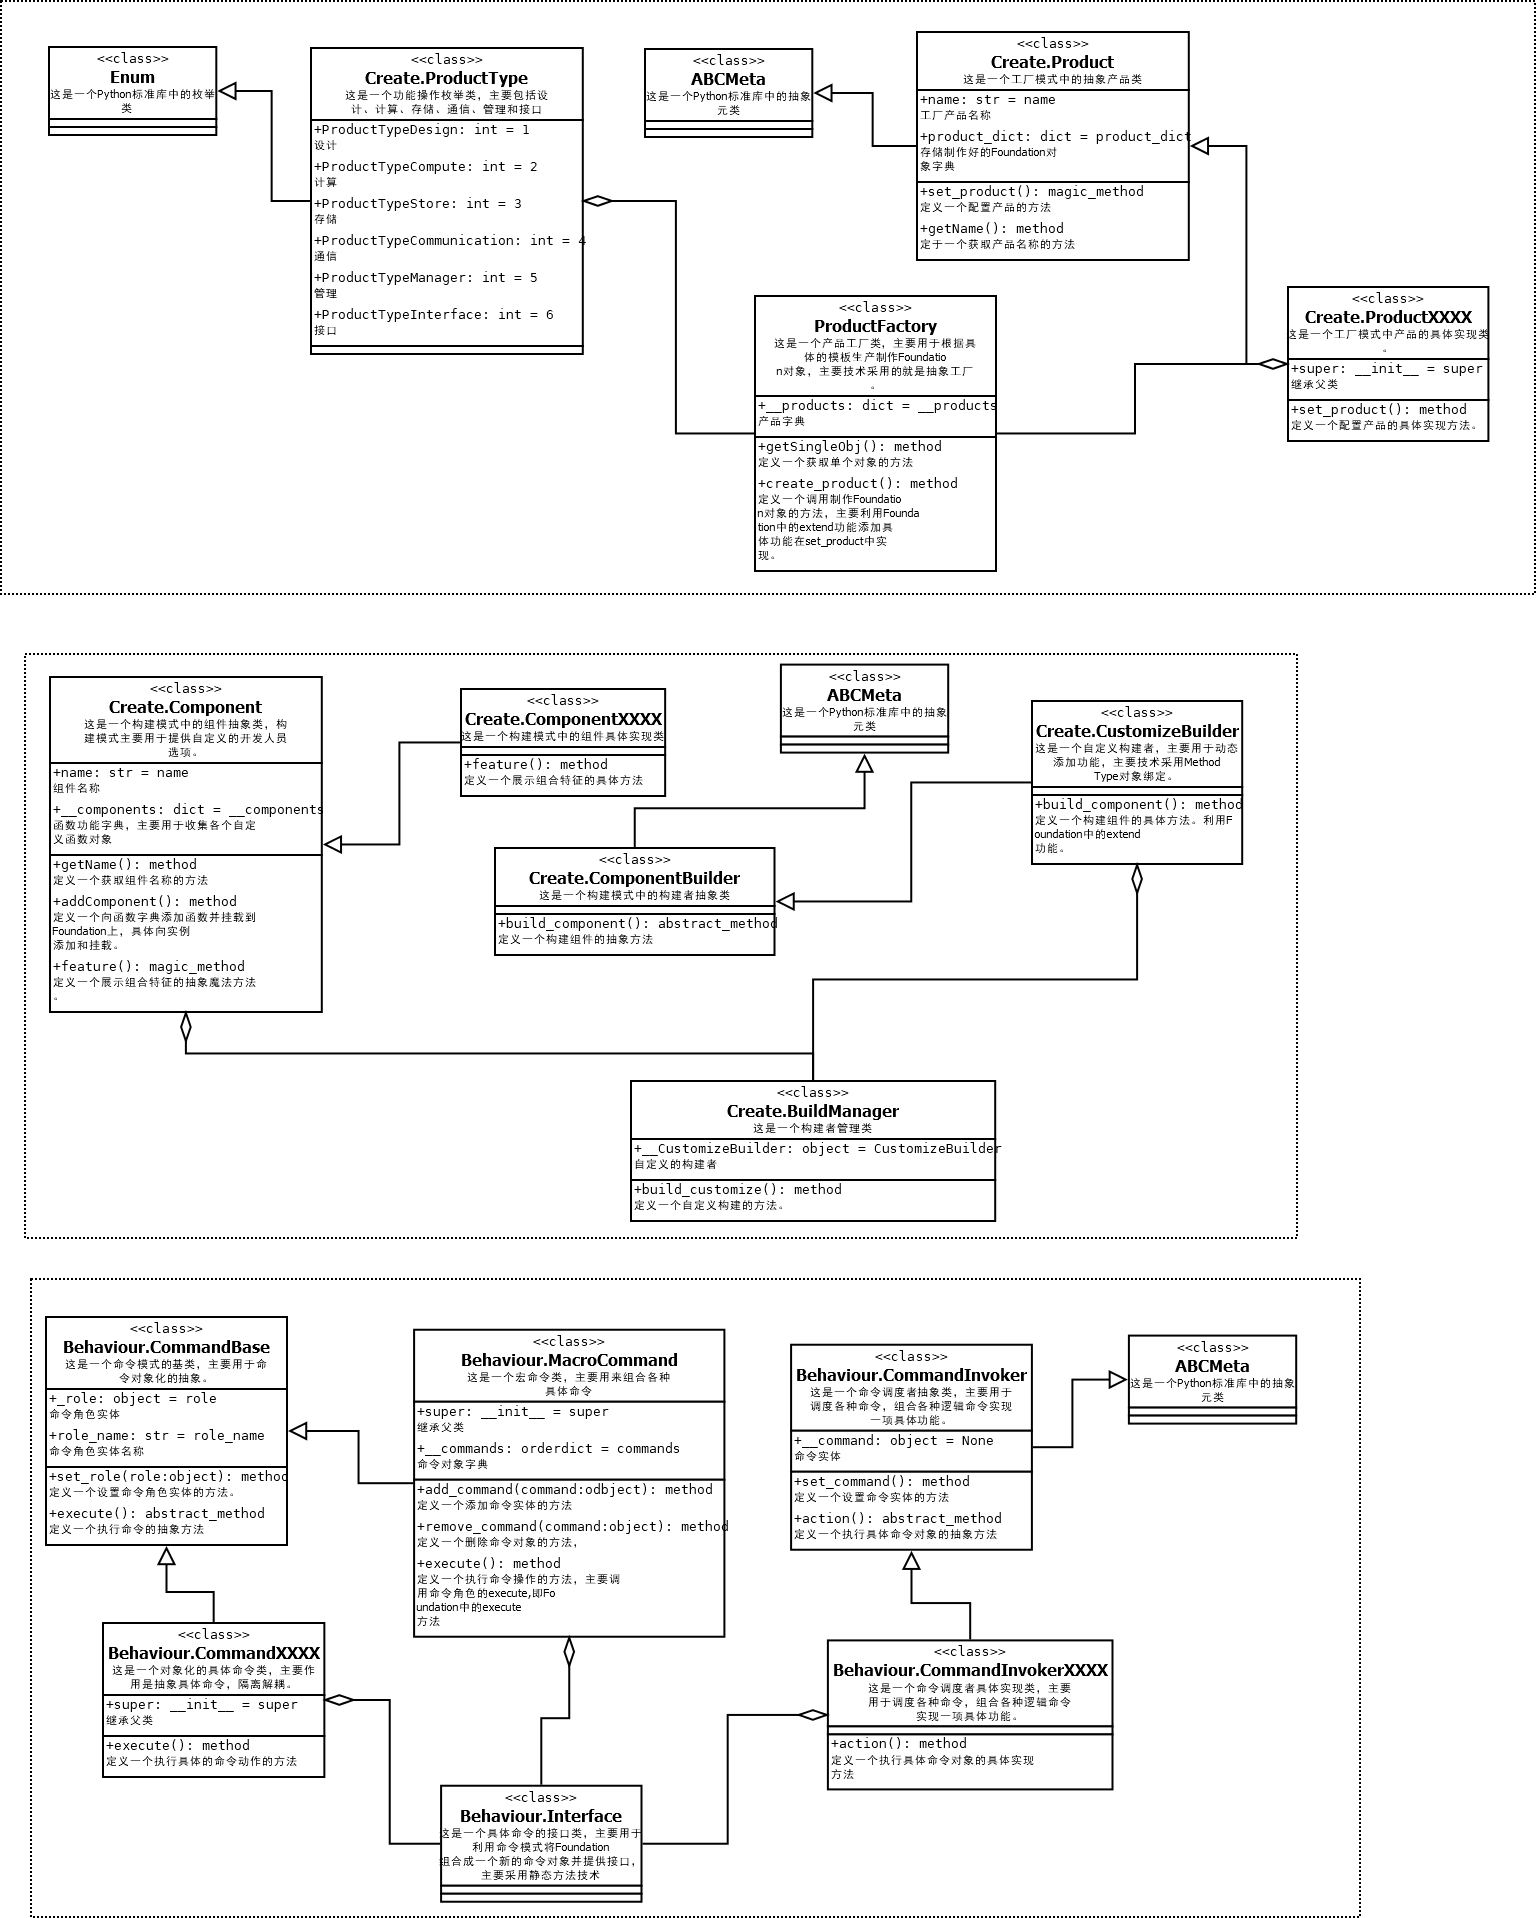
\includegraphics[width=0.8\textwidth]{Controller.png}
}

\centerline{
	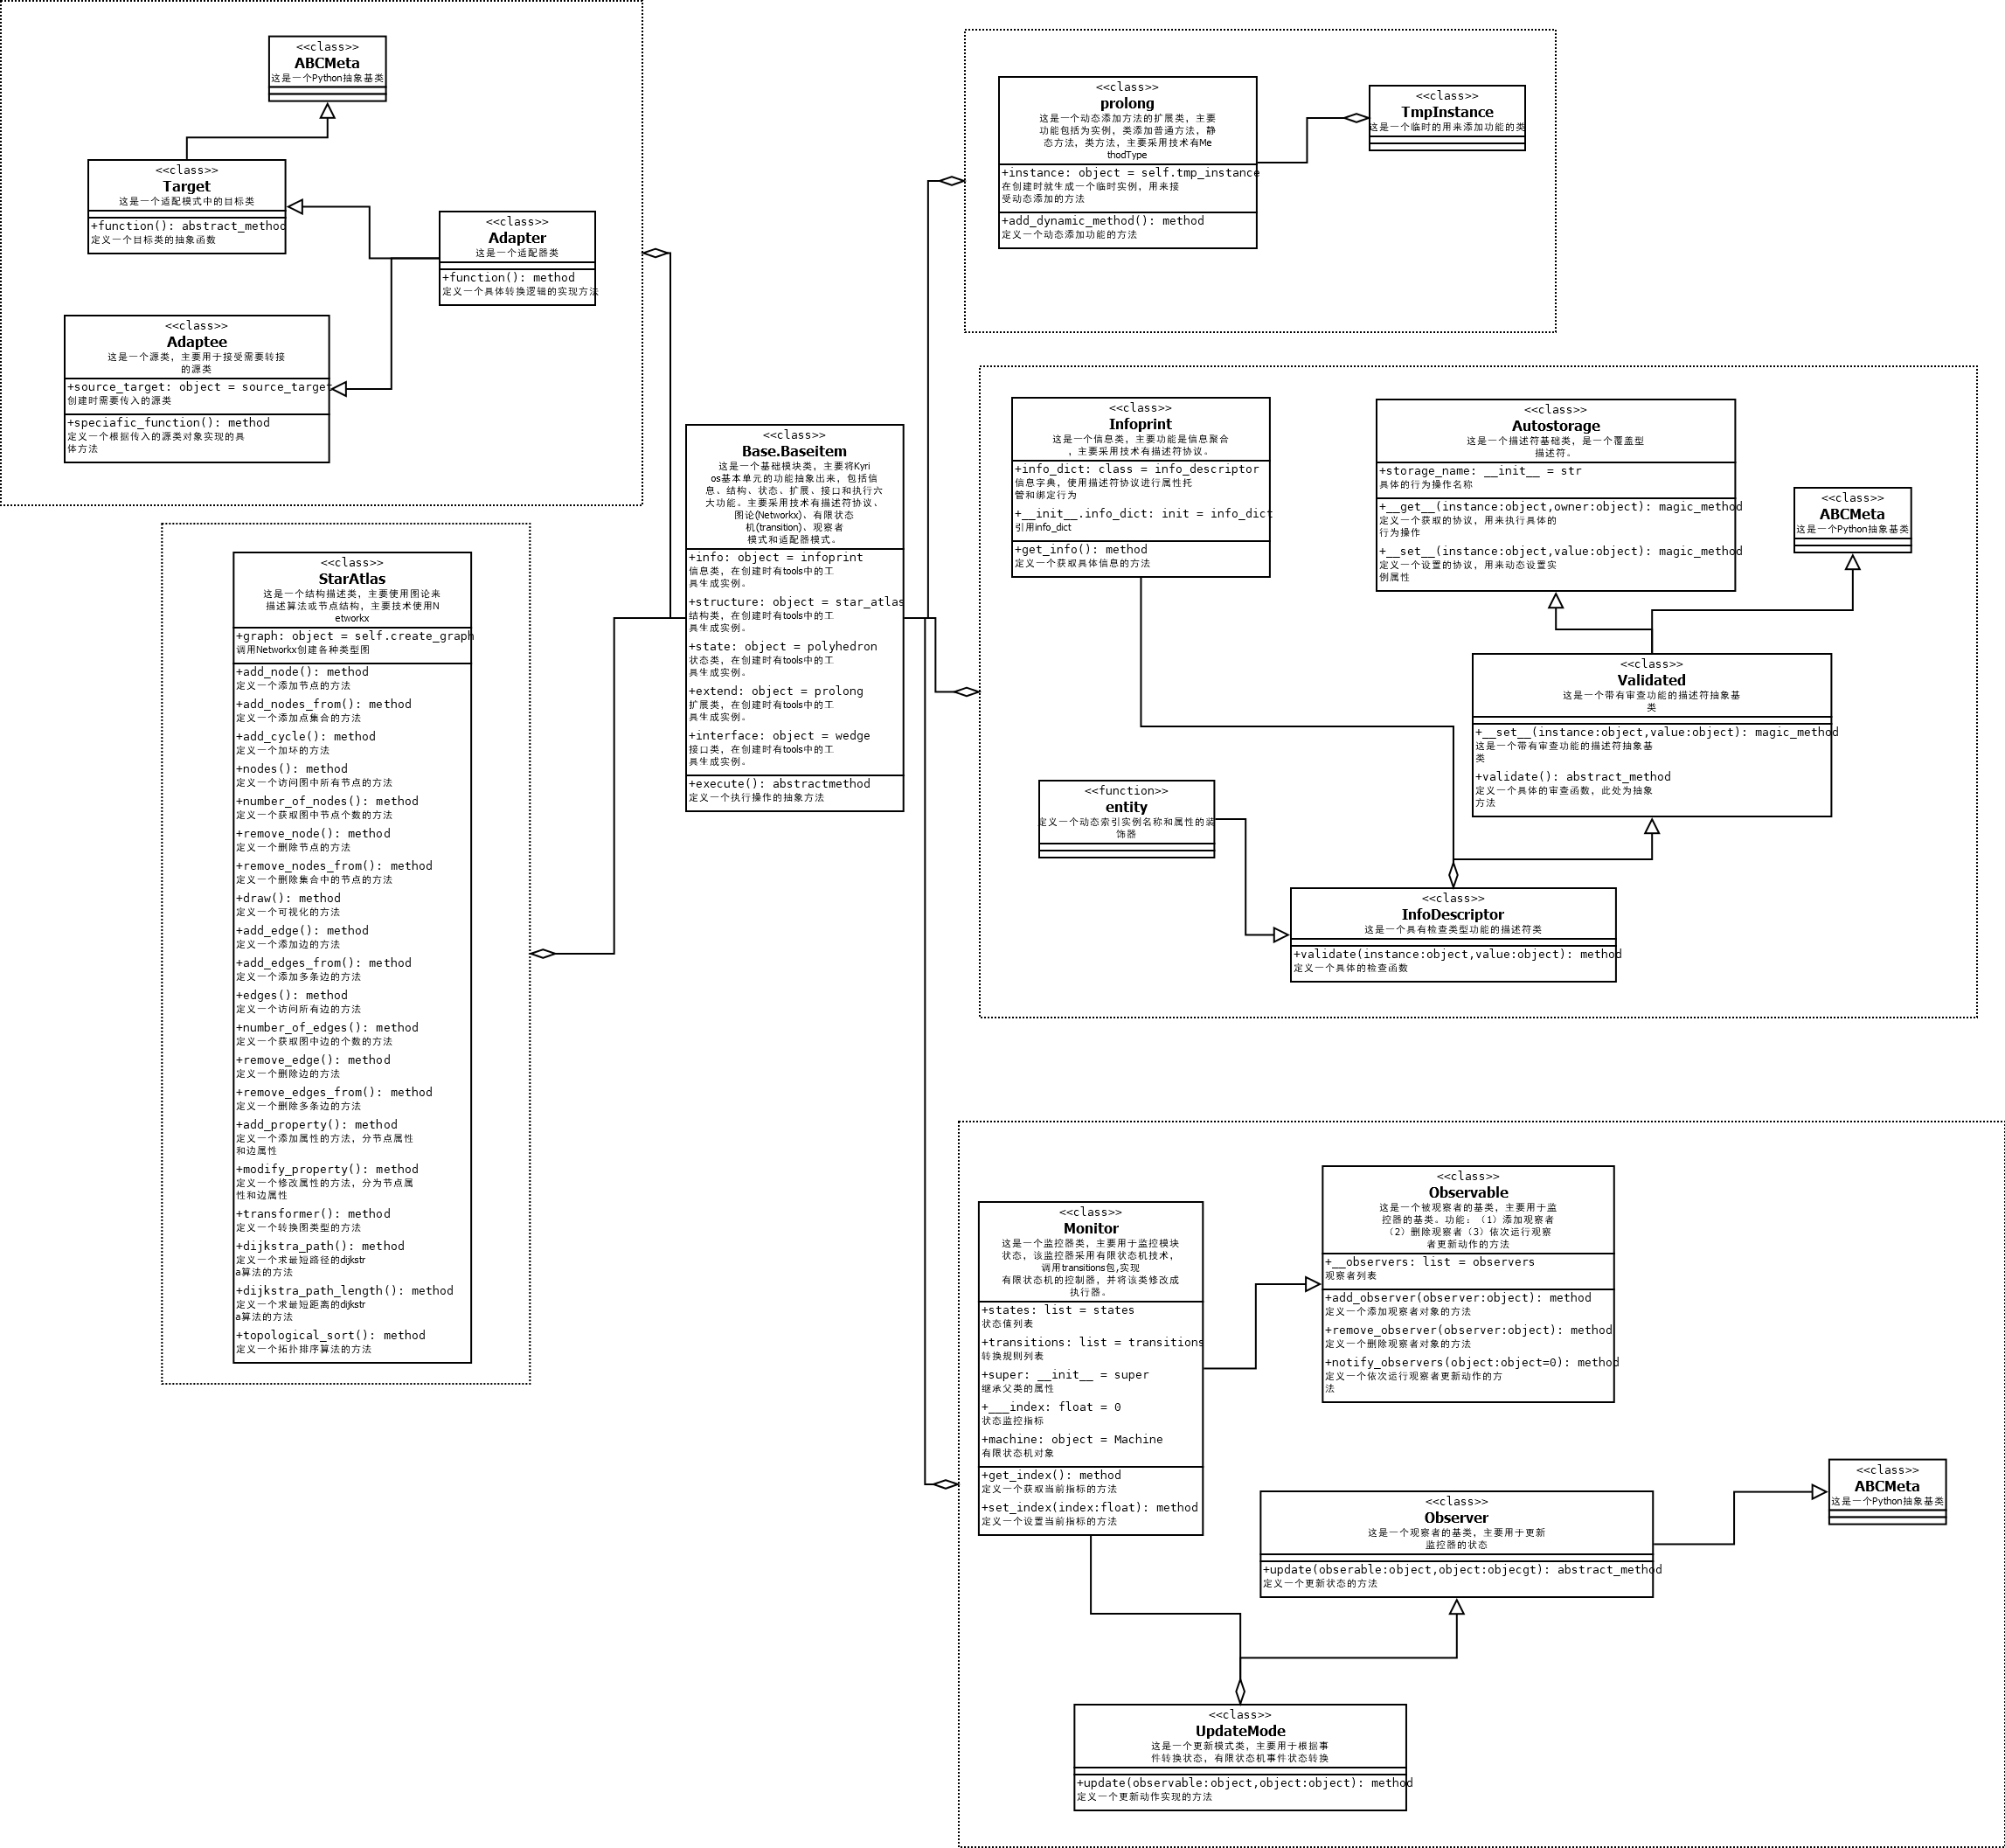
\includegraphics[width=0.8\textwidth]{Extend.png}
}

\centerline{
	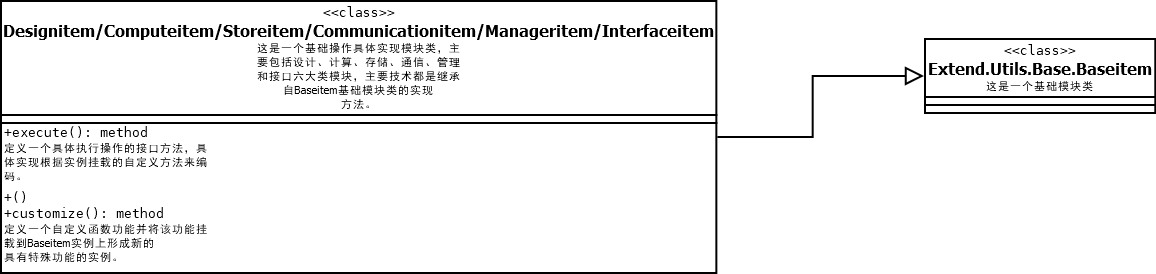
\includegraphics[width=0.8\textwidth]{Foundation.png}
}




\subsection{基础套餐}

基础套餐主要包括计算、存储、管理、通信、设计和接口六大功能。目前采用的技术有Ray,Alluxio,Hydra。目前开放的功能单元如下:



\subsubsection{计算}

计算单元作为算法应用的运行核心,提供算法高效运行方式,如分布式异构计算,实现算法加速。主要涉及的技术有:
\begin{enumerate}[label=\arabic*).]
	\item \textit{Ray}\\
	主要用于分布式计算和进程通信。
\end{enumerate}



\subsubsection{存储}

存储单元作为算法应用的交互核心,提供算法的数据抽象层,实现数据统一格式,加速IO操作。主要涉及的技术有:
\begin{enumerate}[label=\arabic*).]
	\item \textit{Alluxio}\\
	主要用于数据抽象层。
\end{enumerate}



\subsubsection{管理}

管理单元作为算法应用的组织核心,提供算法高效组织方式,实现算法的灵活配置,快速落地生产。主要涉及的技术有:
\begin{enumerate}[label=\arabic*).]
	\item \textit{Hydra}\\
	主要用于动态配置。
	\item \textit{Hydra}\\
	主要用于脚本模板自动生成与配置。	
\end{enumerate}







\subsection{使用示例}

Kyrios的API可分为两级,第一级主要由具体的功能模块自己自主开放出来,第二级由控制模块统一调度开放并提供跨组件自由组合的扩展。当然,两级别的API都具有高度自定义的特性。

代码示例:

\begin{lstlisting}
	from Kyrios.Extend.Base.basic import *
	# from Kyrios.Extend.Tools.state import *
	# from Kyrios.Extend.Tools.structure import *
	# import networkx as nx
	# from Kyrios.Extend.Tools.extend import *
	# from Kyrios.Extend.Tools.interface import *
	from Kyrios.Foundation.Manager.hydra_config import *
	from Kyrios.Controller.Create.factory_mode import *
	from Kyrios.Controller.Create.build_mode import *
	from Kyrios.Controller.Behaviour.command_mode import *
	from Kyrios.Foundation.Function.function_interface import *
	
	
	Baseitem = Baseitem()
	### info测试
	print("======================================================================== (1)info测试")
	Baseitem.info.info_dict = {'1':'测试信息类'}
	print(Baseitem.info.info_dict)
	### state测试
	print("======================================================================== (2)state测试")
	Baseitem.state.FiniteStateMachine.update_mode(' >= 0.6')
	Baseitem.state.FiniteStateMachine.setIndex(0.7)
	print("接收到指标后的状态:",Baseitem.state.FiniteStateMachine.state)
	Baseitem.state.FiniteStateMachine.stop()
	print("运行完成后的状态",Baseitem.state.FiniteStateMachine.state)
	Baseitem.state.FiniteStateMachine.restart()
	print("重新启动:",Baseitem.state.FiniteStateMachine.state)
	### structure测试
	print("======================================================================== (3)structure测试")
	Baseitem.structure.graph.add_edges_from([('n', 'n1'), ('n3', 'n1'), ('n2', 'n3')])
	toposort_list = Baseitem.structure.graph_algorithm(algorithm = 'toposort')
	print(Baseitem.structure.graph.nodes(),toposort_list)
	### extend测试
	print("======================================================================== (4)extend测试")
	from Kyrios.Extend.Tools.tmp import *
	Baseitem.extend.Prolong.add_dynamic_method(set_age,'set_age')
	Baseitem.extend.Prolong.add_dynamic_method(set_sex,'set_sex')
	print(Baseitem.extend.Prolong.show_function())
	Baseitem.extend.Prolong.prolong_instance.set_age(10)
	print(Baseitem.extend.Prolong.prolong_instance.data['age'])
	Baseitem.extend.Prolong.prolong_instance.set_age(20)
	print(Baseitem.extend.Prolong.prolong_instance.data['age'])
	### interface测试
	print("======================================================================== (5)interface测试")
	from Kyrios.Extend.Tools.tmp import *
	def test():
	test_source_target.test()
	Baseitem.interface.Wedge.add_source_target(test_source_target)
	Baseitem.interface.Wedge.function(test,'test')
	Baseitem.interface.Wedge.run_interface('test')
	print(Baseitem.interface.Wedge.function_dict)
	### Foundation测试
	print("======================================================================== (6)HydraConfig测试")
	Hydraitem = HydraConfig()
	Hydraitem.info.info_dict = {'1':'测试信息类'}
	print(Hydraitem.info.info_dict)
	Hydraitem.customize(set_sex,'set_sex')
	Hydraitem.execute(function_name = 'set_sex',sex = 'male')
	print(Hydraitem.extend.Prolong.show_function())
	print(Hydraitem.extend.Prolong.prolong_instance.data['sex'])
	Hydraitem.customize(generate_execute_file,'gen_exec_file')
	print(Hydraitem.extend.Prolong.show_function())
	cmd_tmp = 'python D:\\AEwork\\algorithm_platform\\Kyrios\\Demo\\Kyrios\\Foundation\\Function\\hydra_main.py +db=mysql +algorithm=ai_1'
	Hydraitem.execute(function_name = 'gen_exec_file',cmd = str(cmd_tmp))
	### factory_mode测试
	print("======================================================================== (7)factory_mode测试")
	factory = ProductFactory()
	ProductHydra = factory.create_product(ProductType.ProductTypeManager)
	print(ProductHydra.extend.Prolong.show_function())
	ProductHydra.execute(function_name = 'set_sex',sex = 'female')
	print(ProductHydra.extend.Prolong.show_function())
	print(ProductHydra.extend.Prolong.prolong_instance.data['sex'])
	### build_mode测试
	print("======================================================================== (8)build_mode测试")
	from Kyrios.Extend.Tools.tmp import *
	custom_item = BuildManager()
	custom_item.add_customize_component(set_age,'set_age')
	custom_item.add_customize_component(set_sex,'set_sex')
	custom_item.add_customize_component(set_value,'set_value')
	components = custom_item.show_components('all')
	print(ProductHydra.extend.Prolong.show_function())
	custom_item.mount_component('set_value',ProductHydra)
	print(ProductHydra.extend.Prolong.show_function())
	### command_mode测试
	print("======================================================================== (9)command_mode测试")
	command_interfacer = CommandInterface()
	command_interfacer.add_foundation(ProductHydra,'Hydra')
	return_result = command_interfacer.simple_execute_macrocommand(ProductHydra,function_name = 'set_sex',sex = 'male_male')
	print(return_result)
	### hydra测试
	print("======================================================================== (10)hydra测试")
	factory = ProductFactory()
	ProductHydra = factory.create_product(ProductType.ProductTypeManager)
	print(ProductHydra.extend.Prolong.show_function())
	cmd_tmp = 'python D:\\AEwork\\algorithm_platform\\Kyrios\\Demo\\Kyrios\\Foundation\\Function\\hydra_main.py +db=mysql +algorithm=ai_1'
	ProductHydra.execute(function_name = 'generate_execute_file',cmd = cmd_tmp)
	### ray测试
	print("======================================================================== (11)ray测试")
	cmd_tmp = 'python D:\\AEwork\\algorithm_platform\\Kyrios\\Demo\\Kyrios\\Foundation\\Function\\ray_main.py +db=mysql +algorithm=ray'
	factory = ProductFactory()
	ProductRay = factory.create_product(ProductType.ProductTypeCompute)
	print(ProductRay.extend.Prolong.show_function())
	ProductRay.execute(function_name = 'generate_execute_file',cmd = cmd_tmp)
	### 辅助测试
	print("======================================================================== (12)辅助测试")
	# from ServerManager.ServerCommandInterface import *
	# # minio server test
	# object_file = 'D:\\AEwork\\algorithm_platform\\Kyrios\\TEST\\ray\\tmp_ray.py'
	# tmp_interface = ServerManagerCommandInterface()
	# tmp_value = tmp_interface.PutObject(connect_info = '10.2.12.248:9000',
	#                                                     access_key = 'minioadmin',
	#                                                     secret_key = 'minioadmin',
	#                                                     secure = False,
	#                                                     object_file = object_file,
	#                                                     bucket = 'ray')                                                    
	# print("===============>",tmp_value)
	# SSH_host_dict = {
		# 	'host' : '10.2.12.248',
		# 	'port' : 22,
		# 	'username' : 'shihua',
		# 	'pwd' : 'ATTACK7121553rb1'
		# }
	# command = "cd /home/shihua/tulip/test/ray/;mv 'D:\\AEwork\\algorithm_platform\\Kyrios\\TEST\\ray\\tmp_ray.py' tmp_ray.py"
	# tmp_value = ServerManagerCommandInterface.SSHRunCMD(SSH_host_dict = SSH_host_dict,
	#                                                     command = command)
	# print("===============>",tmp_value)
	### Alluxio测试
	factory = ProductFactory()
	ProductAlluxio = factory.create_product(ProductType.ProductTypeStore)
	print(ProductAlluxio.extend.Prolong.show_function())
	alluxio_client = ProductAlluxio.execute(function_name = 'generate_alluxio_client',host = '10.2.12.248',port = 39999)
	print(alluxio_client.ls('/'))
	print(dir(alluxio_client))
\end{lstlisting}



\end{document}
